\documentclass{article}
% uncomment to set the page format to A4 instead of A5
\def\RELEASEDOCUMENT{}

% preamble
% language and encoding
\usepackage[utf8]{inputenc}
\usepackage[T1]{fontenc}
\usepackage[brazil]{babel}

% fonts: normal and monospaced
\usepackage[charter]{mathdesign}
%\usepackage{mathpazo}
%\usepackage{newtxtext, newtxmath}
%\usepackage[scaled]{ulgothic}
\usepackage{inconsolata}

% page format
\ifdefined\RELEASEDOCUMENT
\usepackage[landscape, a4paper, margin=2cm]{geometry}
\else
\usepackage[landscape, a5paper, margin=0.7cm]{geometry}
\fi

% additional commands to math mode
\usepackage{amsmath}

% indent first line of first paragraph
\usepackage{indentfirst}

% page numbering
\pagestyle{empty}

% automatically format quotes (no need to write as ``'')
\usepackage{csquotes}
\MakeOuterQuote{"}


% support coloured links, PDF bookmarks, etc.
%\usepackage[colorlinks=false, pdfstartview=FitH, pdfpagelayout=OneColumn]{hyperref}

% remove space after a comma when it acts like a decimal separator
\usepackage{icomma}

% "cancel" terms with a slash
%\usepackage{cancel}

% enable use of colours
%\usepackage{xcolor}

% show customised enumerate 
%\usepackage{enumerate}

% support graphics
\usepackage{graphicx}

% input raw text
%\usepackage{verbatim}

% add cells that span more than one row or column
%\usepackage{multirow, multicol}

% include external raw PDF pages
%\usepackage{pdfpages}

% allow forcing force a figure to be displayed "here"
%\usepackage{float}

% input code
%\usepackage{listings} \lstset{basicstyle=\ttfamily}

% add "lorem ipsum" text
%\usepackage{blindtext} \blindmathtrue

% add questions and answers
\usepackage[]{exercise}
\renewcommand{\ExerciseName}{Questão}
\renewcommand{\ExerciseListName}{Q\!\!}
\renewcommand{\AnswerName}{Resposta}
\renewcommand{\AnswerListName}{Resposta}
\renewcommand{\ExePartName}{Item}
\renewcommand{\ExerciseHeader}{\hrule~\par\noindent{\textbf{\large
            \ExerciseName~\ExerciseHeaderNB\ExerciseHeaderTitle
            \ExerciseHeaderOrigin. \medskip}}}
\renewcommand{\ExePartHeader}{~\par\noindent{\textit{\large
            (\ExePartHeaderNB)
            \smallskip}}}
\renewcommand{\theExePart}{\alph{ExePart}}
\renewcommand{\ExePartHeaderNB}{\theExePart}



% add Portuguese trig functions
\DeclareMathOperator{\sen}{sen}
\DeclareMathOperator{\tg}{tg}
\DeclareMathOperator{\cotg}{cotg}
\DeclareMathOperator{\cossec}{cossec}
\DeclareMathOperator{\arcsen}{arcsen}
\DeclareMathOperator{\arctg}{arctg}
\DeclareMathOperator{\arccotg}{arccotg}
\DeclareMathOperator{\arccossec}{arccossec}

% add British commands and environments
\newenvironment{centre}[0]{\begin{center}}{\end{center}}
\newenvironment{itemise}[0]{\begin{itemize}}{\end{itemize}}


\title{
    Engenharia de Software -- Profª Ana C. V. de Melo\\
    Projeto Kindred -- Fase 3
}

\author{
    Bruno Guilherme Ricci Lucas (4460596)\\
    Leonardo Pereira Macedo (8536065)\\
    Vinícius Bitencourt Matos (8536221)
}


\begin{document}
\maketitle

O \emph{use-case} que definimos na primeira fase contempla a criação e realização de
uma partida completa do jogo, o que inviabiliza a criação de um teste para ele. O
mesmo se aplica a um dos \emph{statecharts} definidos na segunda fase, correspondente
a uma partida inteira.

Desta forma, decidimos criar \emph{use-cases} de partes do sistema, de modo a testar
seus componentes.

\section{Dados de teste}

\newcommand{\teste}[3]{
    \item\textbf{#1:}
    \begin{itemise}
        \item\textbf{Entrada: } #2
        \item\textbf{Saída: }   #3
    \end{itemise}
}

\begin{itemise}

\teste
    {testClient\_WrongIP}
    {Um client é criado e manipulado para se conectar a um servidor inexistente:
    um que possui o nome\emph{fakehost}.}
    {A saída esperada seria ocorrer um \texttt{RuntimeException}, mostrando que
    houve erro na conexão com o servidor.}

\teste
    {testClient\_CorrectIP}
    {Um client é criado e manipulado para se conectar a um servidor já previamente
    rodando no \emph{localhost}.}
    {A saída esperada seria não ocorrer um \texttt{RuntimeException}, visto que a
    conexão foi feita com sucesso.}

\teste
    {testQuit}
    {É criado e inicializado um Client, que logo envia um comando para sair.}
    {A saída esperada seria receber uma afirmação positiva do \texttt{assertFalse},
    ou seja, é falso que o Client esteja conectado após o comando \texttt{QUIT}.}

\teste
    {testQuit}
    {É criado e inicializado um Client, que logo envia um comando para sair.}
    {A saída esperada seria receber uma afirmação positiva do \texttt{assertFalse},
    ou seja, é falso que o Client esteja conectado após o comando \texttt{QUIT}.}
    
\teste
    {testNick\_Invalid}
    {Cliente envia \texttt{NICK} (comando de terminal) com os seguintes parâmetros,
    todos inválidos:
        \begin{itemise}
            \item \texttt{aa}
            \item \texttt{3444}
            \item \texttt{abc\%}
        \end{itemise}
    }
    {Espera-se que o \emph{nickname} do cliente não mude em nenhum dos casos. Ou
    seja, que \texttt{client.getNickname()} seja \texttt{null} (valor para
    \emph{nickname} indefinido) em todos os casos testados.}

\teste
    {testNick\_Valid}
    {Cliente envia \texttt{NICK} com o seguinte parâmetro: \texttt{niceNick}, um
    parâmetro válido.}
    {Esperamos que o Cliente de fato recebe e guarde a \emph{string}
    \texttt{niceNick} como seu \emph{nickname}, pois ela é válida.}


\teste
    {testHost\_Invalid}
    {Um Cliente vira \emph{host} de uma partida. Temos três situações disponíveis:
        \begin{enumerate}
            \item Cliente sem \emph{nickname} usando um mapa que não existe. No caso,
                os parâmetros são: \texttt{null} (\emph{nickname}) e
            "\texttt{thisIsFake}" (nome do mapa).
            \item Cliente sem \emph{nickname} usando um mapa válido. No caso, os
                parâmetros são: \texttt{null} e "\texttt{simpleMap}".
            \item Cliente com \emph{nickname} válido usando um mapa inválido. No
                caso, os parâmetros são: "\texttt{hostInvalid}" (um \emph{nickname}
                válido) e "\texttt{thisIsFake}".
        \end{enumerate}
    }
    {Espera-se que os testes nos digam que:
        \begin{itemise}
            \item Em 1, \emph{nickname} e nome de mapa de fato não valem.
            \item Em 2, \emph{nickname} não vale, mas nome do mapa vale.
            \item Em 3, \emph{nickname} vale, mas nome do mapa não.
        \end{itemise}
    }
    
\teste
    {testHost\_Valid}
    {Cliente com \emph{nickname} válido vira \emph{host} de uma partida usando um
    mapa válido. Após um tempo, ele muda para um outro mapa válido. Os parâmetros
    usados são: "\texttt{hostValid}" (\emph{nickname} do \emph{host}),
    "\texttt{simpleMap}" e "\texttt{happyPlains}" (nome dos mapas válidos).}
    {Espera-se que o Cliente de fato sirva de \emph{host} para os mapas escolhidos,
    mesmo após a mudança.}

\teste
    {testUnhost\_Invalid}
    {Há dois casos:
        \begin{enumerate}
            \item Cliente com nickname inválido e sem ser um \emph{host} (não deu o
            comando ou não escolheu um mapa válido) tenta dar \texttt{UNHOST}.
            Neste caso, os parâmetros são nulos.
            \item Cliente com nickname válido e sem ser um \emph{host} tenta dar
            \texttt{UNHOST}. Neste caso, os parâmetros acabam sendo nulos, já que
            não há sala.
        \end{enumerate}
    }
    {Espera-se que, por o Cliente não ser \emph{host}, o comando \texttt{UNHOST} não
    funcione.}

\teste
    {testeHost\_Valid}
    {Cliente com nickname válido começa a ser \emph{host} de uma sala usando um mapa
    válido. Após um tempo, ele dá o comando \emph{unhost}. Os parâmetros são:
    "\texttt{unhostVal}" (nickname) e "\texttt{testmap}".}
    {Espera-se que o Cliente possa se tornar \emph{host} e cancelar o comando sem
    problemas.}

\teste
    {testJoin\_Valid}
    {Dois Cliente são conectados ao servidor com nicknames válidos. Um será o
    \emph{host} e o outro o \emph{guest}. O \emph{host} cria uma sala usando um mapa
    válido e o \emph{guest} entra nela. Os parâmetros são: "\texttt{hostJoin}" e
    "\texttt{guestJoin}" (nomes do \emph{host} e do \emph{guest}) e
    "\texttt{testmap}" (nome do mapa). Em seguida, eles desconectam.}
    {Espera-se que o servidor reconheça que os dois Clientes estão em jogo antes de
    eles se desconectarem.}

A partir daqui, temos os testes para partidas em si. Usaram-se mapas especialmente preparados para testes,  \emph{testmap} (para quase todos os casos) e \emph{testmatch} (para testar o fim da partida), além de uma unidade de debug chamada \emph{Master}.

\teste
    {testSurrender}
    {Dois Clientes, um \emph{host} e um \emph{guest}, se conectam ao servidor e uma
    sala é criada. O jogo começa e o \emph{host} (primeiro a jogar) dá o comando
    \texttt{SURRENDER} para desistir da partida. Logo após os dois se desconectam.
    Os parâmetros são "\texttt{hostSur}" e "\texttt{guestSur}" como nicknames do
    \emph{host} e do \emph{guest} e "\texttt{testmap}" como mapa.}
    {Espera-se que os dois Clientes sejam reconhecidos como "\texttt{isPlaying}"
    até o momento em que o \emph{host} dá o comando \texttt{SURRENDER}. Na
    averiguação subsequente, espera-se que nem o \emph{host} nem o \emph{guest}
    sejam reconhecidos como "\texttt{isPlaying}".}

\teste
    {testEndTurn}
    {Um Cliente é criado e vira um \emph{host}. É verificado o turno (-1). Então um
    \emph{guest} entra na sala e o jogo começa. É verificado o turno (1-turno do
    \emph{host}). O \emph{host} dá o comando endTurn. É verificado o turno (2-turno
    do \emph{guest}). O \emph{guest} dá o comando endTurn. É verificado o turno
    (1-turno do \emph{host}). Os parâmetros são "\texttt{hostEnd}",
    "\texttt{guestEnd}" e "\texttt{testmap}". Além dos já mencionados -1, 1 e 2 para
    as comparações de turno.}
    {Espera-se que de fato os turnos mudem da forma descrita acima.}

\teste
    {testMove\_Valid}
    {Um \emph{host} e um \emph{guest} estão em jogo. O \emph{host} manda a unidade na
    localização 0 0 se mover para a localização 1 0. Após uma pausa ele tenta
    movê-la de novo.}
    {Espera-se que de fato o \emph{host} consiga mover a unidade da primeira vez,
    mas que ele falhe na segunda tentativa.}

\teste
    {testMove\_Invalid}
    {Durante uma partida, um \emph{host} tenta mover uma unidade usando diversos
    comandos inválidos, seja tentando mover uma unidade em uma posição inválida,
    seja tentando colocar uma unidade em uma posição inválida, ou partindo de uma
    posição inválida para tentar posicionar em outra posição inválida. Também é
    testado posicionar uma unidade em uma tile ocupada, ou posicionar em um lugar
    que extrapole o movimento da unidade selecionada, assim como tentar mover
    uma unidade inimiga.}
    {Espera-se que nenhum dos comandos testados sejam aceitos, já que são todos
    inválidos.}

\teste
    {testAttack\_Valid}
    {Durante uma partida, o \emph{host} comanda uma unidade para atacar um inimigo.
    É dada uma pausa e o \emph{host} tenta mover e atacar com a mesma unidade
    novamente. Os parâmetros são "\texttt{hostAtkVl}", "\texttt{guestAtkVl}" e
    "\texttt{testmap}".}
    {Espera-se que a unidade selecionada ataque com sucesso na primeira vez.
    Em seguida, é esperado que o \emph{host} falha em tentar movimentar ela e
    atacar com ela.}

\teste
    {testAttack\_Invalid}
    {Durante uma partida, o \emph{host} tenta atacar. São testadas diversas
    coordenadas inválidas, tiles vazias como sendo alvo, atacar uma unidade além do
    range da unidade sendo usada, atacar usando uma unidade inimiga e atacar uma
    unidade aliada. Os parâmetros são "\texttt{hostAtkIn}", "\texttt{guestAtkIn}" e
    "\texttt{testmap}".}
    {Espera-se que nenhuma das entradas testadas seja bem-sucedida, já que são
    inválidas.}

\teste
    {testUnitsNextTurn}
    {Durante uma partida, um \emph{host} movimenta uma unidade e ataca uma unidade
    inimiga, encerrando seu turno em seguida. O \emph{guest} então encerra seu turno,
    passando a vez para o \emph{host}, que tenta mover uma unidade e atacar usando
    ela. Os parâmetros são "\texttt{hostCtrl}", "\texttt{guestCtrl}" e
    "\texttt{testmap}".}
    {Espera-se que o \emph{host} possa usar suas unidades normalmente após o
    \emph{guest} encerrar seu turno.}

\teste
    {testMatch}
    {Durante uma partida, o \emph{host} destrói todas as unidades adversárias, efetivamente vencendo o oponente.}
    {Espera-se que tanto o \emph{host} quanto o \emph{guest} automaticamente saiam da partida e voltem para o menu principal, onde podem interagir com o servidor e procurar novos oponentes. Curiosamente, o programa passa neste teste, mas notamos que os jogadores ficam travados na partida após o ataque final quando experimentamos com o projeto.}


\end{itemise}

\section{Teste de classes}
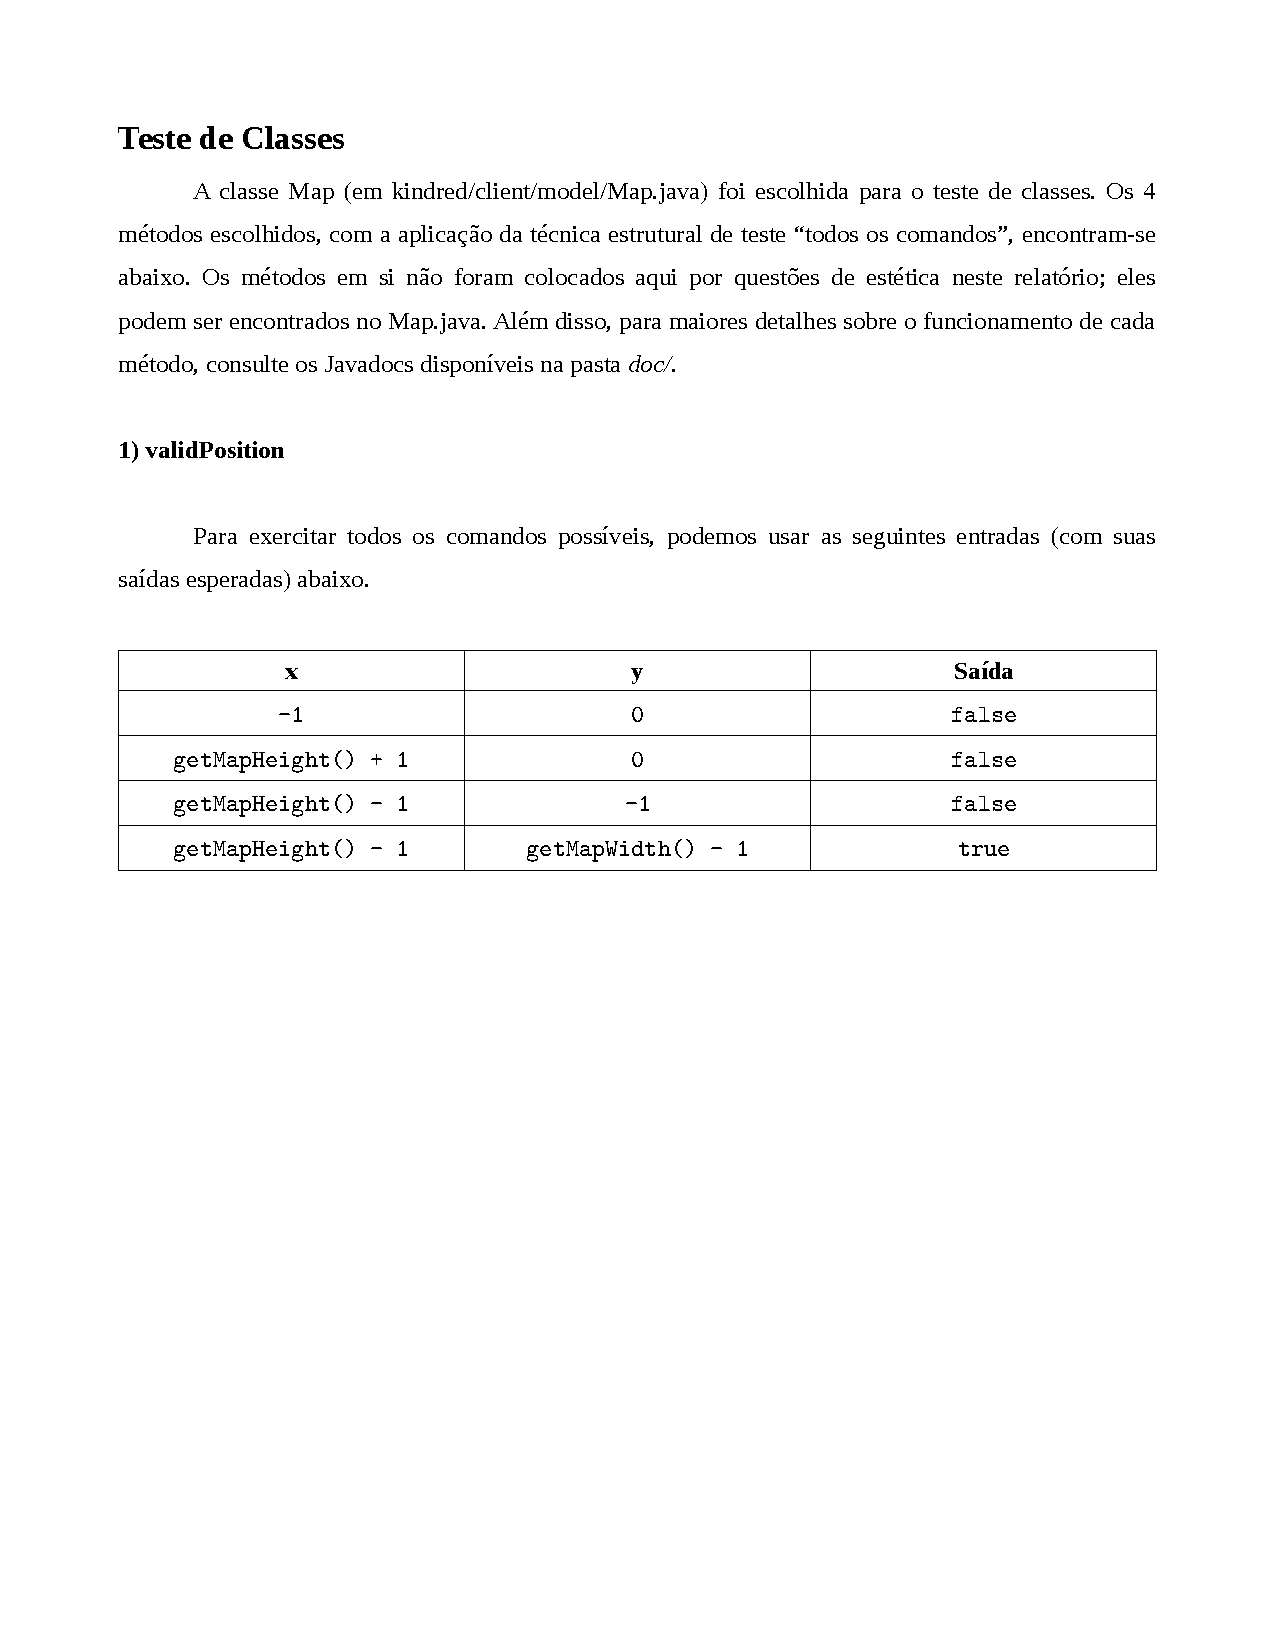
\includepdf[pages=1-]{testeClasses.pdf}
\section{Erros encontrados nos testes}

Tivemos alguns problemas para iniciar os testes. A parte que gerencia as trocas
entre cliente e servidor não estava implementada de uma maneira que permitisse a
produção de testes de uma maneira intuitiva e simples. Tivemos grandes dificuldades
inicialmente, pois não sabíamos exatamente como proceder. Após um tempo, tivemos
a ideia de fazer uma refatoração do código usando o método \emph{test-first}.
Primeiro pensamos nos testes a serem feitos e então passamos a alterar o código
com isso em mente. Com isso, foi muito mais simples retrabalhar o código e gerar
os testes. A maioria foi feita sem grandes dificuldades, excetuando os casos abaixo:

\begin{enumerate}
    \item Comando \texttt{QUIT} fazia com que todos os testes parassem. Foi devido a
        comandos \texttt{System.exit()} no cliente.

       \textbf{SOLUÇÃO:} Retirada de uns \texttt{System.exit()} no cliente,
            deixando-o mais limpo.

    \item Comando \texttt{NICK}, sendo usado simultaneamente por 2 clientes, fazia
        com que o segundo tivesse um erro de \emph{nickname} já definido. Isso
        ocorria devido à estrutura \emph{static} nas \texttt{ClientToServerMessage}s.

       \textbf{SOLUÇÃO:} Refatoração nas mensagens cliente-servidor.

    \item Fim de Partida: Este é um caso à parte. Todos os testes feitos foram
        aprovados, no entanto, ao se jogar o jogo, vemos que ele não tem fim.
        Quando todas as unidades de um dos lados são destruídas, o laço do jogo não
        se encerra, mesmo que seja detectado que não há mais unidades de um dos
        Clientes. Ainda não foi encontrada uma solução para este problema.
\end{enumerate}

\section{Análise comparativa}

Infelizmente, devido aos problemas apresentados no relatório de erros encontrados
durante os testes, a grande maioria dos diagramas que havíamos feito se tornaram
ultrapassados. No entanto, como refatoramos o código pensando nos testes a serem
feitos, acabamos tendo o trabalho simplificado na hora de gerar os testes.

Se não houvesse a necessidade de refatorar o código, não há dúvidas de que os
diagramas que já havíamos gerado serviriam de base para boa parte dos testes, e
esses diagramas nos ajudariam muito no decorrer do desenvolvimento de tais testes.
Fazer testes para \emph{use-cases} em que não há diagramas é algo mais complicado,
visto que é preciso ter uma ótima ideia do funcionamento da implementação a ser
testada.

Em suma, não podemos fazer uma comparação entre a geração de testes para os quais
haviam diagramas e para os quais não haviam, no entanto é do entendimento do grupo
que os diagramas com certeza facilitariam o trabalho.

\section{Problemas no design e na implementação}

Como abordado nos demais relatórios, o grupo precisou refatorar toda a parte do
código responsável por gerenciar as trocas entre cliente e servidor, pois fazer
testes com o código implementado da maneira que estava antes era algo extremamente
complicado. Sendo assim, o grupo agiu para se adequar aos requisitos da Entrega 3. 

Tal refatoração basicamente anulou boa parte dos diagramas de design que havíamos
feito, embora, a um alto nível, alguns ainda pudessem ser utilizados. O jogo em si
era funcional, mas a necessidade de implementar testes falou mais alto.
 
Tendo em vista que há uma seção específica no enunciado para abordar esse assunto,
é claro que algo assim era esperado, o que, sinceramente, não é surpreendente. Foi
a primeira vez que o grupo implementou testes automatizados, e o programa começou
a ser feito antes de nos aprofundarmos nesse assunto em questão durante as aulas.
O grupo todo sabe da importância dos testes e que escrever um programa pensando nos
testes a serem feitos facilita o trabalho em diversos sentidos. É uma lição que
não será esquecida.


\end{document}
